\documentclass[12pt,openright,oneside,a4paper,brazilian]{abntex2}
\selectlanguage{brazil}

\usepackage{capa-epusp-abntex2}

\usepackage[num]{abntex2cite}
\usepackage[utf8]{inputenc}

\usepackage{blindtext}

\usepackage{graphicx}
\usepackage{float}
\usepackage{amsmath}



\title{Warehouse Management System Posicional}

\author{Marco Enrique dos Santos Abensur\\
		Daniel Nery Silva de Oliveira}

\areaconcentracao{Engenharia Elétrica}

\orientador{Gustavo Rehder Pamplona}
\coorientador{Carlos Eduardo Cugnasca}

\preambulo{Trabalho apresentado à Escola Politécnica da Universidade de São Paulo para obtenção do Título de Engenheiro Eletricista.}

\date{São Paulo\\2019}
\pagenumbering{arabic}


\begin{document}

\imprimircapa
\imprimirfalsafolhaderosto
\imprimirfolhaderosto

\begin{resumo}
O estudo de técnicas de localização indoor e outdoor tem crescido muito nos últimos anos. Com a informação da localização de algum ativo em um ambiente controlado, processos podem ser simplificados e dados valiosos podem ser obtidos para os mais variados usos, desde a localização de algum aparelho médico em um hospital, até o de mercadorias em um armazém que é o foco do presente trabalho. Sabendo-se localização de todos os ativos em um armazém, pode-se fazer um uso inteligente desses dados, de forma a otimizar espaço e tempo, o que é essencial para companhias do ramo.
O trabalho será feito em um armazém da \textit{Samsung SDS Cello Logistics} onde as localizações para armazenamento de produtos não são fixas e nem delimitadas. Para solucionar o problema, levando-se em conta custos, eficiência energética e precisão, o uso do Bluetooth low energy 5 (BLE) se mostra como a atual solução mais adequada quando em comparação com outras tecnologias, permitindo precisões de menos de 2m a baixos custos.
%
\\[3\baselineskip]
%
\textbf{Palavras-Chave} -- Indoor Location, Bluetooth Low Energy, Warehouse Managment System.
\end{resumo}


\begin{resumo}[Abstract]
The study of indoor and outdoor localization techniques has grown a lot in recent years. With information about the location of an asset in a controlled environment, processes can be simplified and valuable data can be obtained for a variety of uses, from tracking medical devices in a hospital, to tracking assets in warehouses, which is the focus of this work. With location data of all assets in a warehouse, it is possible to optimize space and time, which is essential for companies in this field.
The work will be done in a warehouse of \textit{Samsung SDS Cello Logistics} where the locations for assets storage are neither fixed nor bounded. In order to solve the problem, taking into account costs, energy efficiency and precision, the use of Bluetooth low energy 5 (BLE) is shown as the most adequate solution when compared to other technologies, allowing for precision of less than 2m and low costs.
%
\\[3\baselineskip]
%
\textbf{Keywords} -- Indoor Location, Bluetooth Low Energy, Warehouse Managment System.
\end{resumo}


\listoffigures
\newpage
% \listoftables
% \newpage

\tableofcontents

\chapter{Introdução}
\textual
A função primaria de um armazém é receber mercadorias de uma fonte, guardar até ser requerido, e enviar para o usuário apropriado quando exigido \cite{tompkins}. É uma parte fundamental da cadeia de suprimentos de qualquer rede de mercadorias.

Nos últimos anos, os armazéns vêm cada vez mais enfrentando maiores demandas por custo e produtividade. Estão se tornando uma parte vital para muitas empresas, porém sua complexidade também está aumentando. Consequentemente, o planejamento e controle dos processos de um armazém, também conhecido como \textit{warehouse management}, tem se tornado uma tarefa desafiadora \cite{faber}.

Nesse contexto, diversas soluções estão sendo buscadas para abaixar os custos, aumentar a produtividade, e melhorar o planejamento dos processos.
Um ponto de melhoria, é a localização de ativos em um armazém. Com dados precisos da localização de todos os ativos em tempo real é possível utilizar algoritmos que visam melhorar a eficiência do armazém.
Os ambientes de armazém, podem ser os mais variados, desde armazéns indoor em ambientes mais controlados, até armazéns outdoor em que espaços são compartilhados entre várias empresas.

Para a realização da localização de produtos em um local indoor e outdoor, diversas tecnologias, técnicas e algoritmos podem ser utilizados, cada um com seus aspectos positivos e negativos, e a escolha de um em detrimento de outro pode levar em conta diversos aspectos. As principais tecnologias utilizadas para a localização são: infravermelho (IR), ultra-som, som audível, sensores magnéticos, sensores óptico, radiofrequência (RF) e luz visível. As tecnologias de RF incluem Bluetooth, banda ultralarga (UWB), wireless sensor network (WSN), rede Local sem fio (WLAN), identificação por radiofrequência (RFID), Near Field Communication (NFC), WiFi, entre outros.
Ja as técnicas de estimativa de localização incluem: Angle of Arrival (AOA), Time of Arrival (TOA), Time Difference of Arrival (TDOA) and Received Signal Strength Indication (RSSI).  \cite{art1,art2}

Essa pesquisa é motivada pela \textit{Samsung SDS Cello Logistics} para a localização de seus ativos em um armazém localizado no Porto de Tubarões no Espirito Santo. Dada a conjuntura do espaço físico de tal porto, somado com os baixos consumos energéticos do Bluetooth, seus baixos custos, e sua alta portabilidade e facilidade de desenvolvimento, tal tecnologia foi escolhida para o desenvolvimento do trabalho, como será demonstrado nas próximas partes.

\chapter{Aspectos Conceituais} 
Esta parte se focará nas mais modernas tecnologias e técnicas para a realização da localização de ativos em um ambiente. Em primeiro lugar é importante fazer uma diferenciação entre a localização de ativos em ambientes outdoor e indoor.

A localização indoor é o termo dado para a localização em ambientes com muitos obstáculos, paredes e teto. Em contraste, a localização outdoor, acontece em ambientes abertos com poucos obstáculo e paredes. Justamente, por introduzir obstáculos, a localização indoor apresenta mais desafios em relação à outdoor. O ambiente em que o trabalho será feito, é um porto a céu aberto, entretanto diversos obstáculos e paredes fazem parte desse ambiente, fazendo do problema mais similar com problemas de localização indoor. geralmente, soluções de localização indoor precisam tomar mais cuidado com precisão, economia de energia, alcance limitado e interferências. Aspectos os quais serão necessários no problema em questão. Tais técnicas, em ambientes sem o obstáculo a mais imposto por um teto, podem alcançar resultados ainda melhores. Dessa forma, a partir de agora, o texto se focará mais no estado-da-arte de tecnologias e técnicas desenvolvidas para ambientes indoor que serão as necessárias para esse trabalho.

\section{Técnicas de localização}
Existe uma variedade de técnicas e algoritmos para obter informações a partir das propriedades de um sinal recebido por um receptor. Os algoritmos usados em sistemas de localização, traduzem as propriedades de um sinal recebido em distâncias e ângulos, os quais são posteriormente usados para o cálculo da localização real de um determinado objeto \cite{art5}. Abaixo uma imagem que resume as principais propriedades de sinal analisadas e os principais algoritmos utilizados para a localização:

\begin{figure}[H]
	\centering 
	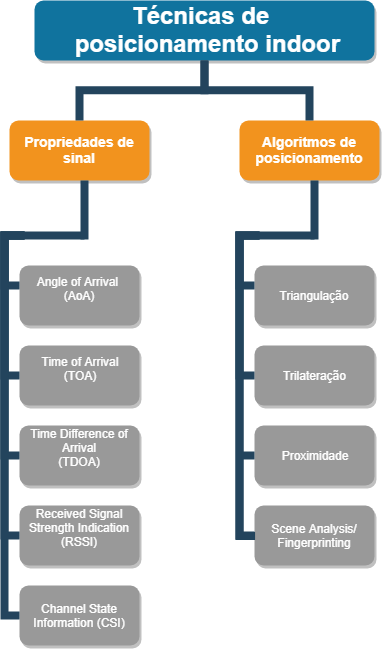
\includegraphics[scale = 0.4]{images/tecnicas_posicionamento_indoor.png}
	\caption{Técnicas localização indoor}
	\label{fig:tecnicas_posicionamento_indoor}
  \end{figure}


\subsection{Angle of Arrival}

Angle of Arrival (AoA), ou em português, ângulo de chegada é o angulo em que o sinal transmitido chega ao receptor. Abordagens baseadas no AoA, usam matrizes de antenas e exploram a diferença de fase das ondas recebidas em cada elemento dessa matriz. E com tal informação é possível estimar o AoA. Na figura \ref{fig:angle_of_arrival} mostra-se uma representação gráfica do processo.

Essa abordagem para estimativa do ângulo de chegada do sinal, geralmente envolve um hardware mais sofisticado quando em comparação com outras propriedades do sinal. Entretanto, com a informação do ângulo de chegada, algoritmos conseguem estimar uma localização com muito mais precisão.\cite{art2}

\begin{figure}[H]
	\centering 
	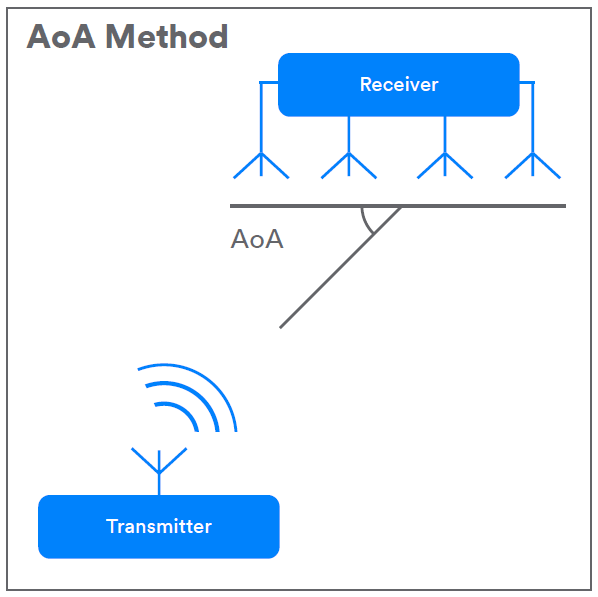
\includegraphics[scale = 0.6]{images/angle_of_arrival.png}
	\caption{Angle of Arrival (AoA)}
	\label{fig:angle_of_arrival}
\end{figure}

\subsection{Time of Arrival (ToA)}

Time of Arrival (ToA) também chamado de  Time of Flight (ToF) é uma técnica que explora o tempo transcorrido para o sinal emitido pelo transmissor chegar ao receptor. Multiplicando-se esse tempo pela velocidade de propagação da luz \(c = 3 \cdot 10^8\) é possível achar a distância entre o sinal recebido e o sinal transmitido. Entretanto essa técnica ainda não é muito precisa, devido as dimensões muito pequenas de tempo envolvidas em aplicaçãoes de curta distância \cite{art6}.

\subsection{Time Difference of Arrival (TDoA)}

Time Difference of Arrival (TDoA) se baseia na diferença nos tempos de propagação de diferentes transmissores, medidos em um receptor, se diferenciando do ToA em que o tempo absoluto é medido. Por essa razão sua complexidade é menor.
nesse método pelo menos 3 transmissores são necessários para determinar a localização do receptor resolvendo-se um conjunto de 3 equações de hipérboles \cite{art2}

\subsection{Received Signal Strength Indication (RSSI)}
Received Signal Strength Indication (RSSI) é a medida do nível de potência do sinal recebido em uma infraestrutura de radiofrequência e pode ser usado para estimação de distâncias.

Usando um modelo simples de propagação de perda de trajetória, a distância d entre transmissor e receptor pode ser estimada a partir de (5.1) como:

\begin{equation} \label{eq:rssi}
RSSI = -10n\log_{10} (d) + A 
\end{equation}

Em que n é o expoente de perda do ambiente (que varia de 2 em um espaço aberto a 4 em ambientes indoor) e A é o valor do RSSI em uma distância de referência do receptor

Entretanto, em ambientes indoor a medição do RSSI e o posicionamento podem ter suas precisões bem reduzidas. \cite{art1}

\subsection{Resumo}
Pode se contruir uma tabela indicando os principais aspectos dos métodos citados:

\begin{figure}[H]
	\centering 
	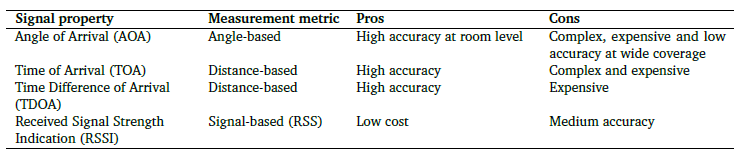
\includegraphics[scale = 1]{images/signal_table.png}
	\caption{Comparação entre técnicas de localização \cite{art1}}
	\label{fig:signal_table.png}
\end{figure}

\section{Algoritmos}

Algoritmos posicionais especificam como calcular a posição de um objeto alvo. Eles traduzem as propriedades dos sinais obtidos em distâncias e ângulos. Os principais algoritmos para localização atualmente são os de triangulação, trilateração, proximidade e o de \textit{scene analysis/fingerprinting}.

\subsection{Triangulação}
Triangulação usa as propriedades geométricas de triângulos para estimar a distância ao alvo por meio da computação de medidas angulares de dois pontos fixos de referência.
A posição de um objeto é encontrada na intercecção de dois pares de linhas de direção de ângulo.
Nesse caso, a propriedade de sinal que está diretamente envolvida é o AoA.

\subsection{Trilateração}
\label{sec:trilateracao}

A trilateração é um algoritmo para estimar a localização de posições desconhecidas baseado nas distâncias relativas para pontos conhecidos \cite{art12}.
Nesse método alguma propriedade do sinal fornece a distância relativa aos pontos conhecidos.

O processo pode ser exemplificado nas imagens abaixo em que as posições A, B e C são conhecidas e a D é desconhecida. Há 4 casos principais que podem acontecer dependendo das distâncias relativas obtidas:

\begin{enumerate}

	\item Circulos se interceptam em um único ponto:
	
	\begin{figure}[H]
		\centering 
		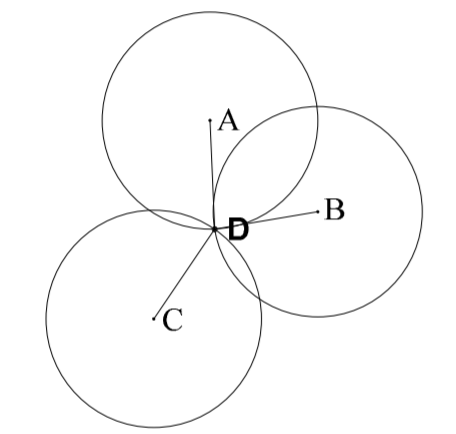
\includegraphics[scale = 1]{images/trilateration.png}
		\caption{Trilateração \cite{art12}}
		\label{fig:trilateration.png}
	\end{figure}
	
	
	As coordenadas podem ser denominadas de \( (x_n, y_n) \) em que n pode ser A, B, C ou D dependendo do ponto em questão. Dessa forma tem-se as seguintes equações:
	
	\begin{equation*}
	\begin{cases} \sqrt{(x - x_a)^2 + (y - y_a)^2} = d_a \\ \sqrt{(x - x_b)^2 + (y - y_b)^2} = d_b \\ \sqrt{(x - x_c)^2 + (y - y_c)^2} = d_c \end{cases}
	\end{equation*}
	
	Resolvendo-se a equação, obtém-se:
	
	\begin{equation*}
	\begin{bmatrix} 
		x \\
		y
	\end{bmatrix} = 
	\begin{bmatrix} 
		2(x_a - x_c) & 2(y_a - y_c) \\
		2(x_b - x_c) & 2(y_b - y_c)
	\end{bmatrix}^{-1}
	\begin{bmatrix} 
		x_a^2 - x_c^2 + y_a^2 - y_c^2 + d_c^2 - d_a^2 \\
		x_a^2 - x_c^2 + y_b^2 - y_c^2 + d_c^2 - d_b^2
	\end{bmatrix}
	\end{equation*}


\end{enumerate}	




\subsection{Proximidade}
É o algoritmo mais simples, entretanto só é utilizado para saber a distância de um objeto de interesse e não sua localização. Por tanto foge do escopo do presente trabalho.


\subsection{Scene analysis/fingerprinting}

Esses métodos se baseiam em coletar préviamente um conjunto de informações do sinal que são únicas a uma deteriminada localidade (\textit{fingerprint}) e posteriormente comparar com o \textit{fingerprint} do alvo. Com técnicas modernas de \textit{machine learning} é possivel encontrar padrões no \textit{fingerprint} de determinado sinal e comparar com posições armazenadas em um banco de dados que possuem \textit{fingerprints} similares \cite{art13}.

Algoritmos baseados nessa técnica são computacionalmente mais caros. Dessa forma o hardware se torna mais complexo. Mas por outro lado, grandes performances podem ser obtidas.

\subsection{Resumo}

Uma tabela pode ser construída comparando os principais pontos positivos e negativos de cada um desses algoritmos.
\begin{figure}[H]
	\centering 
	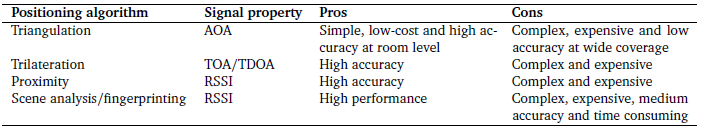
\includegraphics[scale = 1]{images/algorithms_table.png}
	\caption{Comparação entre algoritmos de localização \cite{art1}}
	\label{fig:algorithms_table.png}
\end{figure}

\section{Tecnologias para localização}
Diversas tecnologias têm-se mostrado úteis na função de localização indoor, porém cada um delas tem alguns aspectos positivos e negativos. A seguir se mostrará o estado-da-arte para cada tecnologia de localização. Os principais métodos se baseiam em radio-frequência (como Wi-Fi, Bluetooth, ZigBee, RFID e Ultra Wide Band ), entretanto métodos com luz, visível, ondas acústicas também podem ser utilizados.

\subsection{WiFi}
Wifi opera na banda ISM (Industrial, Scientific and Medical) utilizando principalmente a banda de 2.4GHz. É usada primariamente para a conexão com a internet e tem um alcance que pode chegar a 1Km. A maioria dos dispositivos portáteis são compatíveis com a tecnologia, assim soluções com Wifi não necessita grandes mudanças de infraestrutura. No entanto, interferências na banda ISM acabam afetando a precisão de localização. Além disso, não sendo o foco primário do WiFi a localização, mas sim a comunicação, faltam algoritmos eficientes para a localização.

Alguns trabalhos foram feitos demostrando as capacidades de localização com WiFi a exemplo de \cite{art7}

\subsection{Bluetooth}
Bluetooth é um padrão de tecnologia sem fio para trocar informação entre dispositivos móveis e fixos a curtas distancias. Usa ondas de rádio na banda ISM de 2.4 a 2.485GHz. Bluetooth Special Interest Group (SIG) é a organização responsável pelos padrões da tecnologia.

A última especificação do bluetooth, conhecida como Bluetooh 5.1 foi lançado em Janeiro de 2019, permite alcances de até 350m, velocidades de 2Mbit/s e possui baixo consumo energético \cite{art8}.

A maioria dos sistemas atuais de localização com bluetooth utilizam somente RSSI para estimar a posição, tais métodos atingem precisão entre 1m a 10m. Entretanto, a última especificação do Bluetooth, introduziu AoA, e testes iniciais mostram que a precisão para a localização utilizando algoritmos adequados pode chegar na ordem de centímetros \cite{art9}.

Outro ponto importante do Bluetooth é sua alta compatibilidade com dispositivos atuais. Devido a todos esses fatores, estima-se que até 2022 400 milhões de dispositivos de localização baseados em bluetooth sejam vendidos por ano \cite{art9}.

Um ponto negativo, é que o sinal de RSSI é reportado ao usuário com um intervalo de tempo grande, o que dificulta a localização em tempo real com tal tecnologia.

\subsection{ZigBee}

ZigBee é uma tecnologia sem fio desenhada para ser de baixo custo, ter baixa velocidade de dados e ter eficiência energética. Apesar de ser favorável para a localização em redes sem fio, não está disponível na maioria de dispositivos atuais, fazendo a tecnologia não ser favorável para localização indoor. \cite{art2}

\subsection{Ultra-Wideband (UWB)}
Ultra-wideband é uma tecnologia de comunicação que trabalha com bandas muito largas quando em comparação com outras tecnologias similares. As bandas passam de 500 MHZ. Tais bandas permitem uma série de vantagens como uma maior confiabilidade, ja que o sinal possui diversas componentes de frequência, o que aumenta a possibilidade de que pelo menos algumas passem por obstáculos \cite{art10}.
Além disso, devido aos pulsos de baixa duração (\(<\) 1ns) permitem métodos precisos de localização utilizando ToF, com precisão de centímetros. Desse modo é uma tecnologia promissora para a localização indoor.

Entretanto, o progresso lento do padrão de UWB tem limitado a adoção em larga escala da tecnologia.


\subsection{Sinais sonoros e ultrassônicos}

Utiliza-se sinais acústicos para a localização, de forma similar as tecnologias de radio-frequência.
A principal técnica utilizada é a de ToF, como as ondas de som se propagam a velocidades menores que as eletromagnéticas, tal método apresenta menores desafios em sua implementação. A precisão pode chegar na ordem de centímetros \cite{art11}.

Os maiores problemas são que na faixa audível potencias baixas tem que ser utilizadas para não causar uma poluição sonora. E a faixa audível é a com mais compatibilidade para microfones dos atuais \textit{smartphones}. Já para ondes ultrassônicas, o maior problema, consiste no fato de que a velocidade do som muda de acordo com a temperatura e umidade. Além disso, para ondas sonoras, sons ambientes podem causar uma grande interferência no sistema.


\subsection{Resumo}
A seguinte tabela foi tirada de \cite{art2} com um resumo dos principais pontos de cada tecnologia. Algumas tecnologias não foram citadas em detalhes no presente texto:

\begin{figure}[H]
	\centering 
	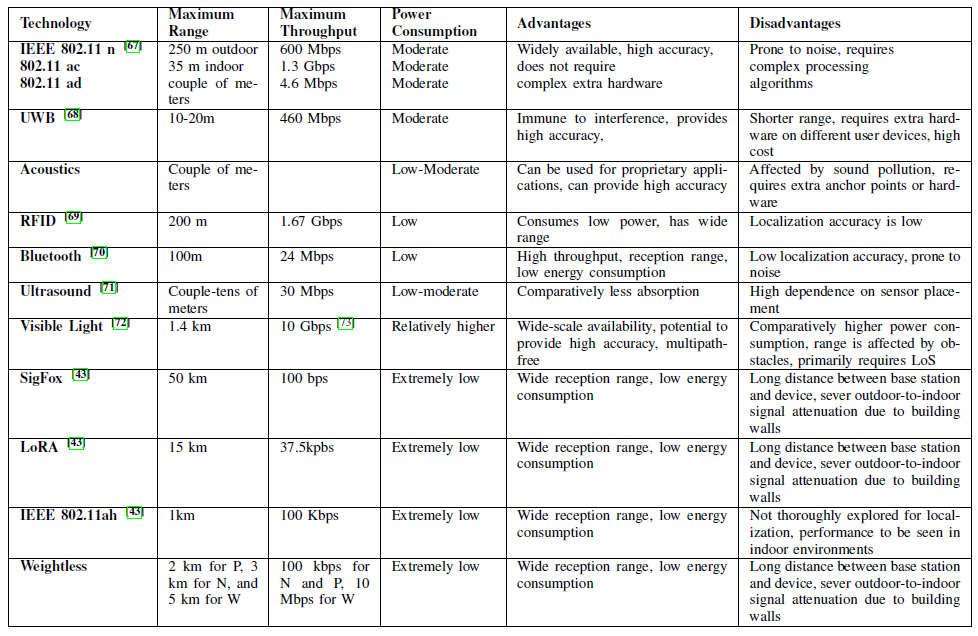
\includegraphics[scale = 0.7]{images/technologies_table.png}
	\caption{Comparação entre tecnologias possíveis para localização. Tirado de \cite{art2}}
	\label{fig:technologies_table}
\end{figure}

\chapter{Tecnologias Utilizadas}

\section{Tecnologia de comunicação}
A partir de todo o levantamento teórico e considerando-se o contexto do problema, a tecnologia que mostrou mais destaque, foi o Bluetooth. 

Mais especificamente, a indrodução do Bluetooth Low Energy (BLE) tornou tal tecnologia bem favorável ao uso para localização, devido ao seu baixo consumo energético, mantendo caracteristicas similares de comunicação.

As principais características da escolha podem ser encontradas abaixo:\newline

\textbf{Economia e eficiência energética} \newline
Uma das principais vantagens da tecnologia Bluetooth para a localização indoor é sua alta eficiência energética. O custo da instalação de um sistema com BLE é baixo quando em comparação de outras tecnologias já que um dispositivo equipado com um chip de BLE pode de 1 a 2 anos com uma unica bateria moeda (\textit{coin cell}).No contexto de um armazém, a economia de custos é fundamental. \newline

\textbf{Acessibilidade e Escalabilidade} \newline
Como mencionado, estima-se que até 2022 400 milhões de dispositivos de localização baseados em Bluetooth sejam vendidos por ano \cite{art9}. Fazendo-o uma tecnologia prontamente acessível e com vários recursos de desenvolvimento.

Para o contexto do projeto, uma rápida implementação é desejável. Além disso, estar presente em dispositivos atuais é um requisito, dado que se deseja a instalação do sistema com o minimo de mudança na infraestrutura atual. Bluetooth está presente na maioria dos telefones celulares, os quais poderiam se integrar ao sistema prontamente. \newline

\textbf{Precisão}\newline
A precisão necessária é tal que dois SKUs (Unidade de Manutenção de Estoque) em localidades diferentes possam ser diferenciados. Para isso, uma precisão de até 1m é desejada.

Com a tecnologia Bluetooth e os algoritmos corretos tal precisão pode ser alcançada.\newline

\textbf{Latência}\newline
A latência no Bluetooth é elevada quando comparada à outras tecnologias. Para aplicações que precisão de localização em tempo real pode ser uma desvantagem. Entretanto no projeto em questão os ativos ficam estáticos no armazém. E a latência não se torna um problema tão grande.\newline

\section{Propriedades do sinal}
Os principais algoritmos mencionados anteriormente exigem para sua implementação uma distância conhecida e um ângulo conhecido para um ponto de referência. No presente trabalho, será utilizado o RSSI para estimar a distância e o AoA para estimar o ângulo.

Quando um chip de Bluetooth recebe o sinal ele é capaz de retornar o valor da intensidade desse sinal, então a obtenção do RSSI é direta e não exige nenhum hardware adicional. Apesar de não ser o método mais preciso para estimar distância, seu custo benefício é alto.

Já para estimar o ângulo, será utilizado o AoA. Tal propriedade em conjunto com a de intensidade do sinal permite que algoritmos estimem uma localização com uma precisão muito maior quando em comparação a algoritmos que utilizam apenas a intensidade do sinal. Assim, apesar de necessitar de um hardware mais complexo, o ganho é alto.

Nas especificações do Bluetooth anteriores à 5.1 lançada em janeiro de 2019, a obtenção do AoA exigia um hardware extra.
Entretanto, dados os recentes avanços na tecnologia agora é possivel estimar o ângulo de chegada de um sinal se o chip Bluetooth utilizado possuir suporte para Bluetooth 5.1 ou superior.

Uma alternativa para estimar o AoA para especificações anteriores à 5.1 é a utilização de um interferômetro de 6-portas, que é um dispositivo que é baseado nas superposições deslocadas de fase das ondas incidentes e refletidas em uma porta. Diferentes defasagens de fase resultam em diferentes potências nas portas de saída da arquitetura de um 6-portas \cite{art14}.

Abaixo um desenho esquemático da arquitetura de um 6-portas: 

\begin{figure}[H]
	\centering 
	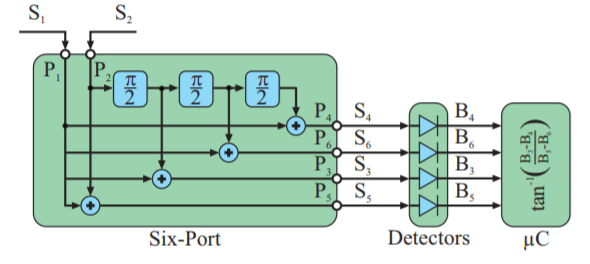
\includegraphics[scale = 1]{images/six_port_schematic.png}
	\caption{Esquemático de uma arquitetura 6-portas. Tirado de \cite{art15} }
	\label{fig:six_port_schematic}
\end{figure}

Na figura \ref{fig:six_port_schematic} os símbolos \( S_1 \) e \( S_2 \) representam os de sinais de entrada e \( S_3 \) a \( S_6 \) representam as potências medidas na saída. Já os simbolos de \( B_3 \) a \( B_6 \) representam as potências de \( S_3 \) a \( S_6 \) convertidas para tensões de base.

As equações que relacionam esses sinais são:

\begin{align*}
    S_3 & = 0.5(S_1 + jS_2) & B_3 = \left | S_3 \right | ^2\\
    S_4 & = 0.5(S_1 - jS_2) & B_4 = \left | S_4 \right | ^2\\
    S_5 & = 0.5(S_1 + S_2)  & B_5 = \left | S_5 \right | ^2\\
    S_6 & = 0.5(S_1 - S_2)  & B_6 = \left | S_6 \right | ^2
\end{align*}

A partir disso, é possível encontrar diversas propriedades úteis dos sinais incidente, tais como a a diferença de fase \( \Delta\phi\), a distância do sinal \( \Delta\delta\) e a propriedade que mais interessa para o presente trabalho, o ângulo de chegada \(\theta\) a partir das seguintes equações:

\begin{equation}
    Z = (B_5 - B_6) + j(B_3 - B_4)
    \end{equation}

\begin{equation}
    \Delta \phi = \arctan \left ( \frac{B_3-B_4}{B_5-B_6} \right )
    \end{equation}

\begin{equation}
    \Delta d = \lambda \frac{\arg\left ({Z}  \right ) }{4\pi }
    \end{equation}

\begin{equation} \label{eq:eq_AoA}
    \theta = \sin^{-1}{(\frac{\lambda \Delta \phi}{2\pi a} )}
    \end{equation}

Em que Z é um número complexo que relaciona as tensões de saída, \(\lambda\) é o comprimento de onda do sinal e \(a\) a distância entre antenas receptoras.

A referência \cite{art15} apresenta um maior detalhamento da arquitetura. Para o contexto de localização indoor, as equações forneceriam o ângulo \(\theta\) desejado.

\section{Prova de Conceito}
Para validar o projeto final, foi proposta uma prova de conceito que aplica as tecnologias mencionadas para obter uma estimativa de distância a partir do Bluetooth.
No projeto final algoritmos, e técnicas mais elaboradas serão utilizados para uma maior precisão, porém na prova de conceito, é possível validar o projeto e mostrar os potenciais de atingir o objetivo final do projeto.

A seguir um detalhamento de como foi elaborada a prova de conceitos e os resultados atingidos.

\subsection{Hardware}
O Hardware escolhido para prova de conceito é a placa de desenvolvimento nRF52840 DK da fabricante de componentes Nordic Semiconductor \cite{nRF52840_site}.

Tal placa de desenvolvimento conta com o SoC nRF52840 que possui Bluetooth 5.0 integrado, e pinos de GPIO com entrada analógica, além de um amplo suporte de recursos online para o desenvolvimento. Soma-se a isso, sua compatibilidade com o SoC nRF52811 da mesma fabricante, que é um dos unicos chips atualmente que possui Bluetooth 5.1 e planeja-se utilizar na etapa final do projeto \cite{nRF52811_site}.

Como o nRF52840 DK não possui suporte para AoA, e placas de desenvolvimento do nRF52811 serão disponibilizadas somente no próximo semestre pela Nordic Semiconductor, pretende-se utilizar um interferômetro de 6-portas desenvolvido no departamento de sistemas eletrônicos da escola politécnica da USP para estimar o ângulo de chegada.

O interferômetro possuí 4 saídas analógicas. Fazendo-se a leitura dessas 4 saídas e utilizando a equação \ref{eq:eq_AoA} encontra-se o AoA.

\begin{figure}[H]
	\centering 
	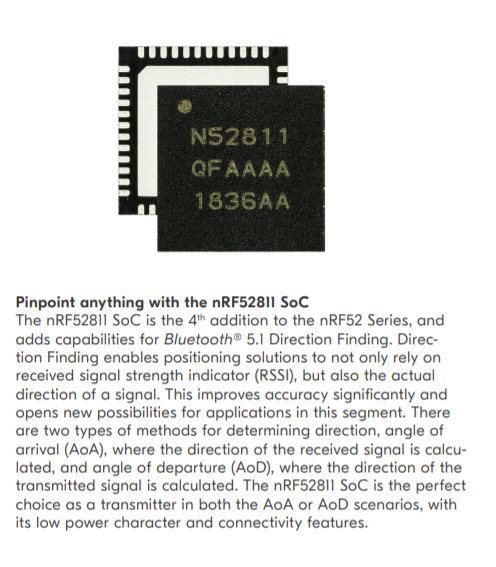
\includegraphics[scale = 1]{images/nRF52811.png}
	\caption{nRF52811. Tirado de \cite{nRF52811_site}}
	\label{fig:nRF52811}
\end{figure}


\begin{figure}[H]
	\centering 
	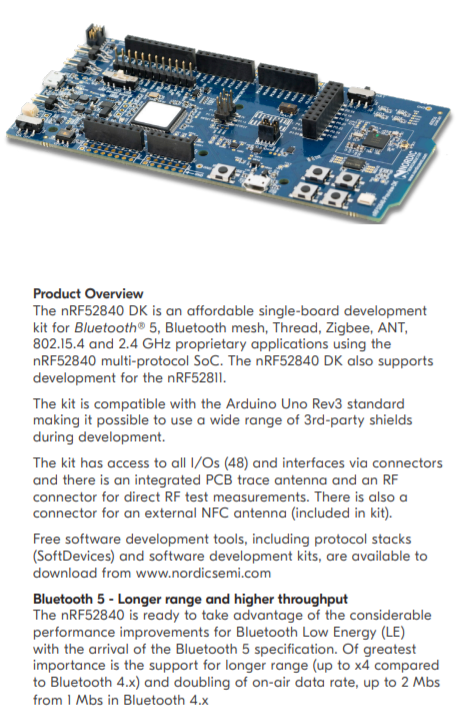
\includegraphics[scale = 1]{images/nRF52840_dk.png}
	\caption{nRF52840. Tirado de \cite{nRF52840_site}}
	\label{fig:nRF52840_dk}
\end{figure}


\subsection{Programa}
A placa de desenvolvimento, na prova de conceito foi programada para procurar dispositivos Bluetooth nas proximidades que tivessem um determinado ID no pacote de \textit{advertising}. Caso fosse encontrado, cada instante que houvesse uma mudança de mais de 5dbm na intensidade do sinal, este era imprimido em uma porta serial.

Além disso, utilizou-se a equação \ref{eq:rssi} para estimar a distância do sinal recebido. O valor para o fator de perda utilizado foi de \(n = 4\) e adotou-se o valor de \(A = -45dbm\).

O dispositivo que emitia o sinal Bluetooth a ser lido foi um celular Samsung Galaxy S8 com Bluetooth 5.0 e um aplicativo pronto que permitia a configuração de um ID específico para um \textit{advertising} a ser enviado.

No programa, o ângulo de chegada ainda não foi implementado

\begin{figure}[H]
	\centering 
	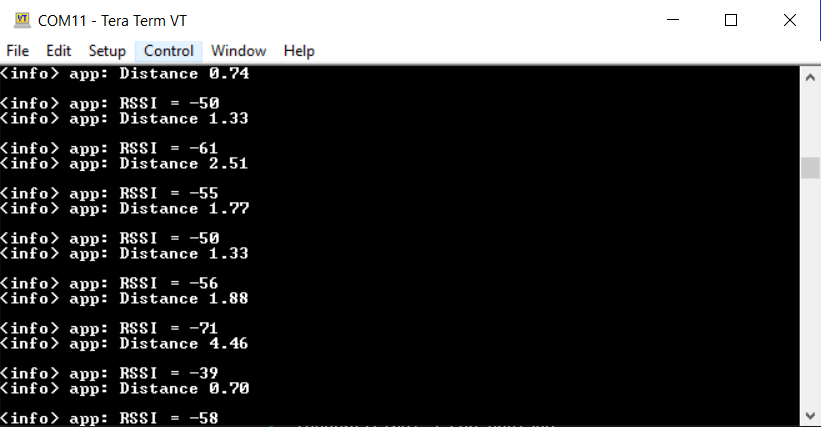
\includegraphics[scale = 0.85]{images/rssi_terminal.png}
	\caption{Porta serial do nRF52840 imprimindo valores de RSSI recebidos}
	\label{fig:rssi_terminal}
\end{figure}

\subsection{Arranjo Experimental}
O arranjo experimental, consistiu em fazer medições de distâncias reais de 0.5m em 0.5m em um ambiente fechado e compará-las com as distâncias estimadas pelos programas e hardware descritos, como se observa na seguinte figura:

\begin{figure}[H]
	\centering 
	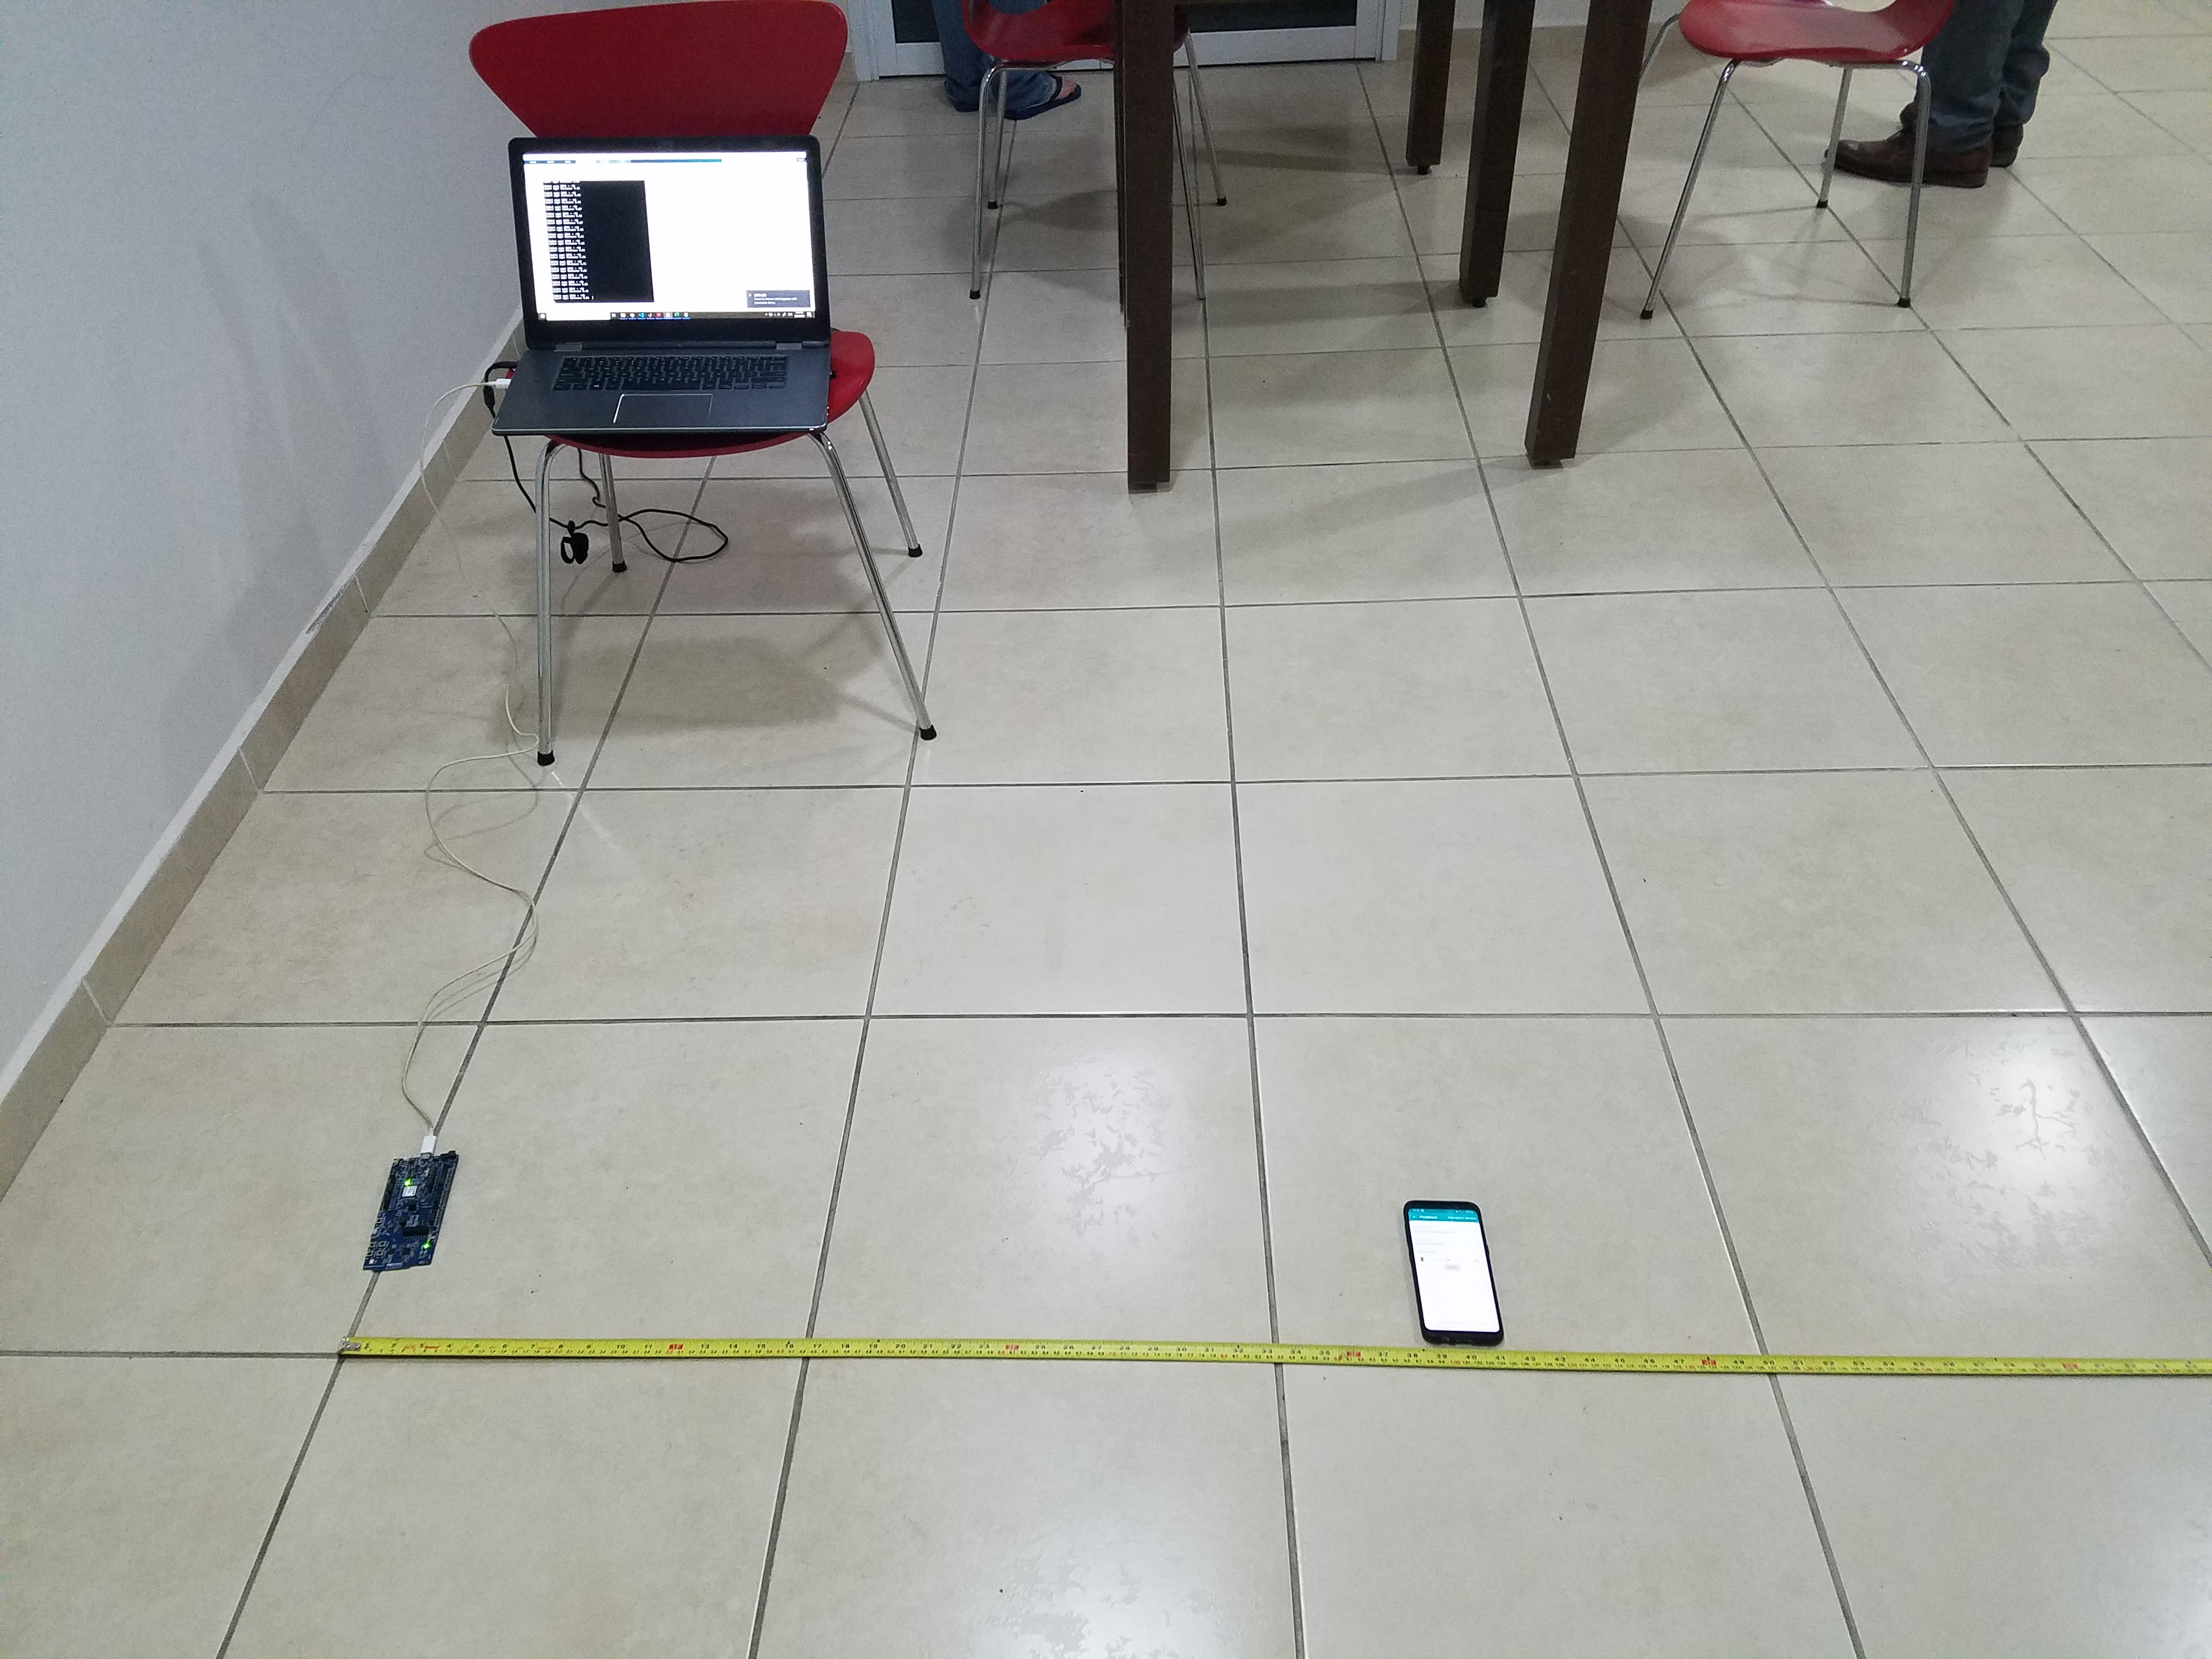
\includegraphics[scale = 0.1]{images/setup_poc.jpg}
	\caption{Arranjo experimental da prova de conceito}
	\label{fig:setup_poc}
\end{figure}


\subsection{Resultados}

Com os dados obtidos, foi possível construir os seguintes gráficos que evidenciam a precisão obtida.
Nota-se que a distância estimada é uma média de 10 leituras diferentes do celular na mesma posição.

\begin{figure}[H]
	\centering 
	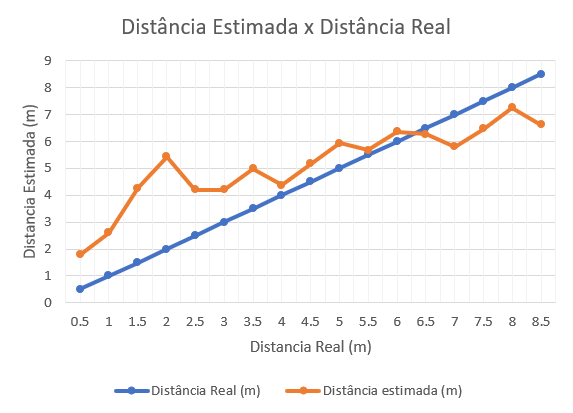
\includegraphics[scale = 1]{images/grafico_distancias_1d.png}
	\caption{Distância Estimada x distância real na prova de conceito}
	\label{fig:grafico_distancia_1d}
\end{figure}

\begin{figure}[H]
	\centering 
	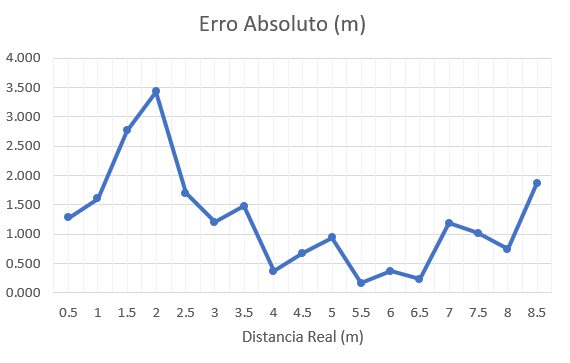
\includegraphics[scale = 1]{images/grafico_erro_1d.png}
	\caption{Erro absoluto em metros em cada distância}
	\label{fig:grafico_erro_1d}
\end{figure}

Deste modo, pelos gráficos apresentados, nota-se que a precisão fica na ordem de 1m a 10m. Tais resultados foram obtidos com o algoritmo mais direto possível e somente utilizando a intensidade do sinal recebido. Ao se introduzir algoritmos mais robustos, a exemplo dos que usam \textit{fingerprint} e AoA, a precisão encontrada será ainda maior.

Ainda como prova de conceito. Simulou-se um sistema de localização 2D utilizando-se somente RSSI e as medidas obtidas anteriormente de distância linear.
Estimou-se uma distância de 5m entre placas, sendo que a placa 1 está na coordenada (0,0) e a placa dois na coordenada (5,0).
Fazendo-se simplificações para o caso 2D na equação \ref{eq:rssi} e substituindo-se os valores, as equações para obter coordenadas em tal sistema são:

\begin{equation}
    x = \frac{a^2 - b^2 + 25}{10} 
\end{equation}
\begin{equation}
    y = \sqrt{a^2 - x^2}
\end{equation}

Em que \(a\) é a distância para a placa na posição (0,0) e \(b\) a distância para a placa da posição (0,5).

Os resultados obtidos a partir disso foram:

\begin{center}
    \begin{tabular}{||c c c c c c c c c||} 
    \hline
    a Real 1 & b Real 2 & a 1 & b 2 & x Calc & y Calc	& x Real & y Real & Erro\\ [0.5ex] 
    \hline\hline
    1 & 5 & 2.61 & 5.94 & -0.34 & 2.58 & 0.10 & 0.99 & 1.64\\ 
    \hline
    2 & 5 & 5.43 & 5.94 & 1.92 & 5.07 & 0.40 & 1.95 & 3.47\\ 
    \hline
    3 & 2.5 & 4.21 & 4.20 & 2.50 & 3.38 & 2.77 & 1.15 & 2.24\\ 
    \hline
    3 & 5 & 4.21 & 5.94 & 0.74 & 4.14 & 0.90 & 2.86 & 1.29\\ 
    \hline
    3 & 7.5 & 4.21 & 6.48 & 0.07 & 4.20 & -2.22 & 2.01 & 3.16\\ 
    \hline
    4 & 1 & 4.37 & 2.61 & 3.72 & 2.29 & 4.00 & 0.00 & 2.30\\ 
    \hline
    4 & 2.5 & 4.37 & 4.20 & 2.64 & 3.48 & 3.47 & 1.98 & 1.71\\ 
    \hline
    4 & 5 & 4.37 & 5.94 & 0.88 & 4.27 & 1.60 & 3.66 & 0.94\\ 
    \hline
    4 & 7.5 & 4.37 & 6.48 & 0.20 & 4.36 & -1.52 & 3.69 & 1.84\\ 
    \hline
    5 & 1 & 5.94 & 2.61 & 5.34 & 2.60 & 4.90 & 0.99 & 1.66\\ 
    \hline
    5 & 2.5 & 5.94 & 4.20 & 4.26 & 4.14 & 4.37 & 2.42 & 1.72\\ 
    \hline
    5 & 5 & 5.94 & 5.94 & 2.50 & 5.38 & 2.50 & 4.33 & 1.05\\ 
    \hline
    5 & 7.5 & 5.94 & 6.48 & 1.82 & 5.65 & -0.62 & 4.96 & 2.53\\ 
    \hline
    6 & 1 & 6.37 & 2.61 & 5.87 & 2.47 & 6.00 & 0.00 & 2.47\\ 
    \hline
    6 & 2.5 & 6.37 & 4.20 & 4.79 & 4.19 & 5.47 & 2.46 & 1.85\\ 
    \hline
    6 & 5 & 6.37 & 5.94 & 3.02 & 5.60 & 3.60 & 4.80 & 0.98\\ 
    \hline
    6 & 7.5 & 6.37 & 6.48 & 2.35 & 5.92 & 0.47 & 5.98 & 1.88\\ 
    \hline
    7 & 2.5 & 5.81 & 4.20 & 4.11 & 4.10 & 6.77 & 1.77 & 3.53\\ 
    \hline
    7 & 5 & 5.81 & 5.94 & 2.34 & 5.31 & 4.90 & 4.99 & 2.57\\ 
    \hline
    7 & 7.5 & 5.81 & 6.48 & 1.67 & 5.56 & 1.77 & 6.77 & 1.21\\ 
    \hline
    8 & 5 & 7.25 & 5.94 & 4.22 & 5.89 & 6.40 & 4.80 & 2.43\\ 
    \hline
    8 & 7.5 & 7.25 & 6.48 & 3.55 & 6.32 & 3.27 & 7.30 & 1.01\\ [1ex] 
    \hline
   \end{tabular}
   \end{center}

   Da tabela, observa-se que mesmo no caso 2D os erros absolutos continuam na faixa de 1m a 10m utilizando-se somente o RSSI.







   
   



\bibliographystyle{abntex2-num}
\bibliography{bibliografia}

\end{document}
